\section{Parameters of the Radiative Transfer Model}
The input parameters of the radiative transfer model (RTM) are the opacity formalisms for the various atmospheric constituents, the index of refraction for each atmospheric layer, the temperature-pressure profiles, and the vertical abundance profiles for the absorbing constituents. Together the last two make up the Thermo-Chemical model of the atmosphere.
\subsection{Temperature-Pressure Profiles}
The temperature-pressure profiles for the atmosphere of Venus have been obtained from the data collected using the Pioneer-Venus sounder and north probes \cite{Seiff-1980}. Figure \ref{fig:temp} shows the temperature as a function of altitude in the Venus atmosphere as reported by the Pioneer-Venus sounder and north probes. Figure \ref{fig:pres} shows the pressures as a function of altitude in the Venus atmosphere as reported by the Pioneer-Venus sounder and north probes.

The sounder probe temperature represents the temperature-pressure profile in the equatorial region of the Venus atmosphere. It is used for latitudes between $-45^\circ$ and $+45^\circ$. The north probe is representative of the polar regions of Venus and it used between $\pm 45^\circ$ and $\pm90^\circ$. A physical surface temperature of 730 K is assumed in this RTM.

\begin{figure}[p]
    \centering
	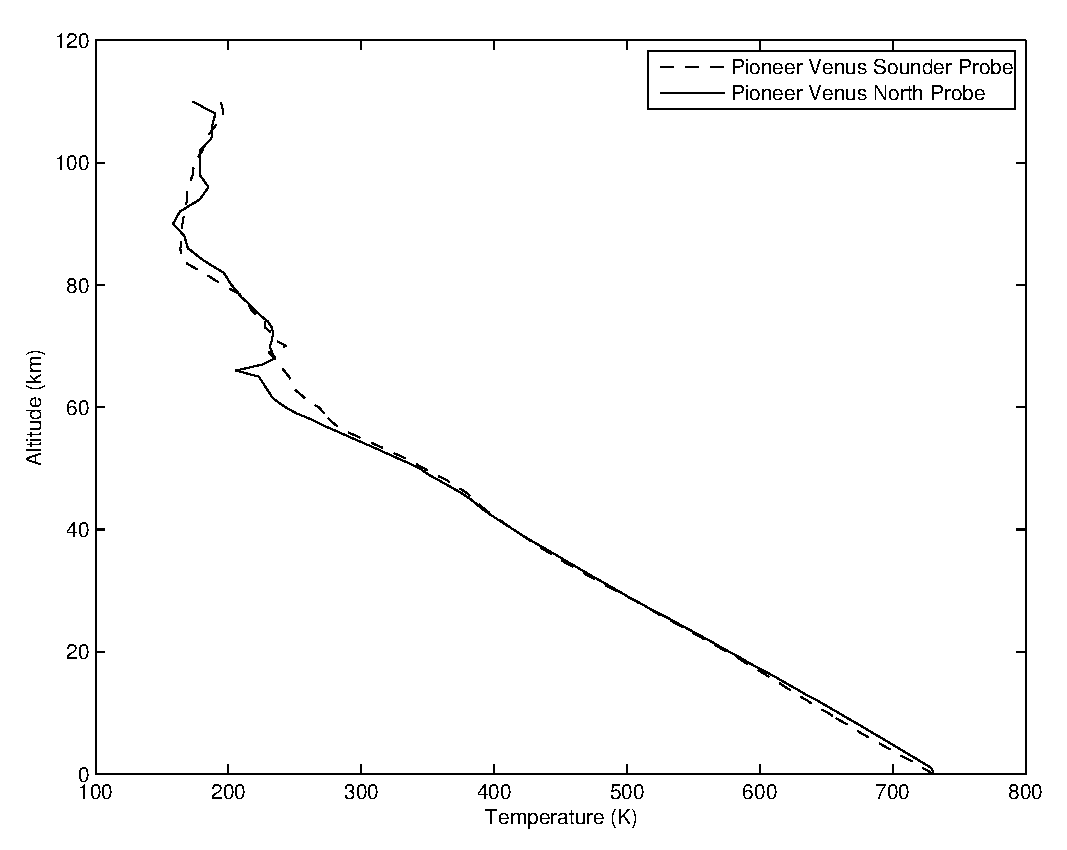
\includegraphics[width=0.7\textwidth]{./rtm/plots/alt-temp.eps}
	\caption{Temperature as a function of altitude in the Venus atmosphere obtained using the Pioneer-Venus sounder and north probes }
		\label{fig:temp}
\end{figure}
\begin{figure}[p]
    \centering
	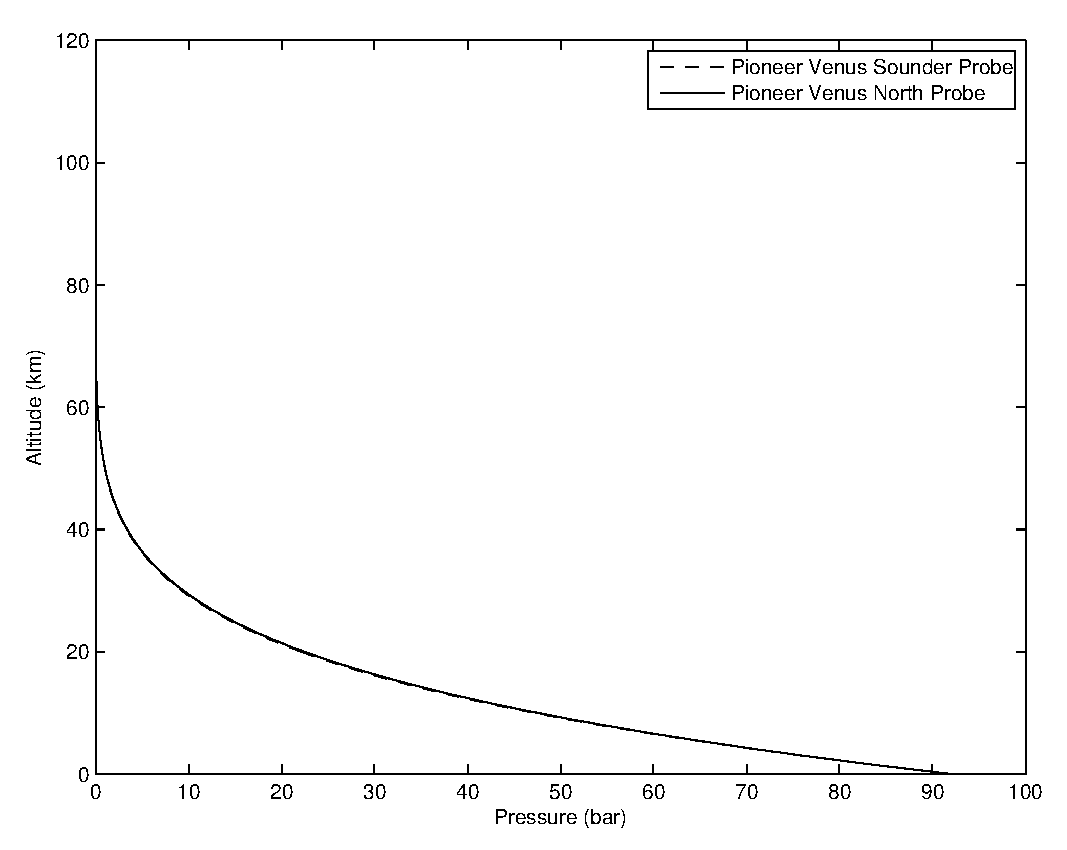
\includegraphics[width=0.7\textwidth]{./rtm/plots/alt-pres.eps}
	\caption{Pressure as a function of altitude in the Venus atmosphere obtained using the Pioneer-Venus sounder and north probes }
		\label{fig:pres}
\end{figure}

\subsection{Opacity Formalisms}

There are several major absorbing constituents at the microwave and millimeter-wave frequencies in the Venus atmosphere. The major constituents are gaseous CO$_2$, N$_2$, SO$_2$, and H$_2$SO$_4$, and liquid H$_2$SO$_4$ in the form of clouds. The formalisms used in this RTM are described below.
\subsubsection{Gaseous CO$_2$-N$_2$}
Although CO$_2$ is a non-polar molecule, collision induced absorption by gaseous CO$_2$ \cite{Barrett-1960} is the dominate source of centimeter- and millimeter-wavelength absorption at low altitudes of the Venus atmosphere. The opacity from gaseous CO$_2$ and N$_2$  was derived by Ho et al. \cite{Ho-1966} based on their laboratory measurements of gaseous CO$_2$-N$_2$. The CO$_2$ and N$_2$ opacity formalism used in this RTM is
\begin{equation}\label{eq:rtm-co2n2}
\alpha_{CO_2} = 1.15\times 10^8(q_{CO_2}^2 + 0.25q_{CO_2}q_{N_2} + 0.0054q_{N_2}^2)f^2p^2T^{-5}
\end{equation}
where $f$ is the frequency in GHz, $p$ is the pressure in atm, T is the temperature in Kelvin, q is the number mole fraction, and $\alpha$ is the absorption in dB/km.

\subsubsection{Gaseous SO$_2$}
The second major opacity contribution comes from gaseous SO$_2$. In the developed RTM, the opacity formalism developed by Fahd and Steffes \cite{Fahd-1991} is described below. The formalism developed by Fahd and Steffes was chosen over the Ben Reuven formalism by Sulieman et al. \cite{Suleiman-1996} due to it's better performance when compared to laboratory measurements as shown previously in this work.

This formalism is based on the Van Vleck-Weisskopf formalism where the contribution from each rotational resonant line to the absorption at a particular frequency can be expressed as 
\begin{equation}
\label{eq:rtm-so2fahd}
\alpha = \alpha_{max} \left(\frac{f}{f_0}\right)^2 \gamma [((f_0-f)^2+\gamma^2)^{-1}+((f_0+f)^2 + \gamma^2)^{-1}]
\end{equation}
where $\alpha_{max}$ is the absorption at the line centers, $f$ is the frequency of interest, $f_0$ is the resonant line frequency, and $\gamma$ is the line width. As per Fahd and Steffes \cite{Fahd-1991} a line width of $\gamma_{SO_2/CO_2} = 7MHz/Torr$ is used for the CO$_2$ broadening of SO$_2$ and a line width of $\gamma_{SO_2/SO_2} = 16MHz/Torr$ is used for the self broadening of SO$_2$. Thus the formalism includes the effects of both CO$_2$ broadening and SO$_2$ self-broadening so that
\begin{equation}
\gamma = \gamma_{SO_2/CO_2}P_{CO_2} + \gamma_{SO_2/SO_2}P_{SO_2}
\end{equation}
where $P_{CO_2}$ and $P_{SO_2}$ are the partial pressures (in Torr) of gaseous CO$_2$ and SO$_2$ respectively.

\subsubsection{Gaseous H$_2$SO$_4$}
The next opacity contribution comes from gaseous H$_2$SO$_4$. The formalism for the opacity of H$_2$SO$_4$ is based on a multiplicative expression fit to laboratory measurements done by Kolodner et al. 1997 \cite{Kolodner-thesis}. There are six best fit expressions based on the frequency of the observation. The formalism is listed below
\begin{eqnarray}
\alpha_{H_2SO_4}(f = 2.26) &=& 106.575 \times q_{H_2SO_4}P^{1.333}\left(\frac{553}{T}\right)^{3.2} \\
\alpha_{H_2SO_4}(f = 8.4)  &=& 451.760 \times q_{H_2SO_4}P^{1.283}\left(\frac{553}{T}\right)^{3.0} \\
\alpha_{H_2SO_4}(f = 11.9) &=& 744.170 \times q_{H_2SO_4}P^{1.309}\left(\frac{553}{T}\right)^{2.9} \\
\alpha_{H_2SO_4}(f = 21.6) &=& 1972.783 \times q_{H_2SO_4}P^{1.08}\left(\frac{553}{T}\right)^{3.0} \\
\alpha_{H_2SO_4}(f < 12)   &=& 33.837 \times q_{H_2SO_4}P^{1.333}f^{1.27}\left(\frac{553}{T}\right)^{3.0} \\
\alpha_{H_2SO_4}(f)        &=& 55.874 \times q_{H_2SO_4}P^{1.333}f^{1.15}\left(\frac{553}{T}\right)^{3.0} 
\end{eqnarray}
where $f$ is the frequency, $q_{H_2SO_4}$ is the mixing ratio of gaseous H$_2$SO$_4$, $P$ is the pressure in atm, and $T$ is the temperature in Kelvin. This RTM implements all of the previously listed formalisms based on the appropriate frequency.

\subsubsection{Liquid H$_2$SO$_4$}
The formalism for the opacity of clouds is taken from Fahd \cite{Fahd-thesis} and is
\begin{equation}
\alpha_{cloud} = \frac{246 M \epsilon_r''}{\rho \lambda \left[ (\epsilon_r' +2)^2 + (\epsilon''_r)^2\right]}
\end{equation}
where $\rho$ is the density of the liquid sulfuric acid (1.84E9 mg/m\^{}3), $M$ is the bulk density of the cloud (50 mg/m\^{}3), $\lambda$ is the wavelength in km and $\epsilon_r'$ and $\epsilon_r''$ are the real and imaginary parts of the complex dielectric constant of the liquid which is found using
\begin{equation}
\epsilon_r = 3.3+\frac{84.2}{\left(1+(2\pi f (1.7\times 10^-11\right))^{0.91}}
\end{equation} 
with f if the frequency in Hz. 
Since clouds are only formed between 48-50 km the absorption is only appropriate for the temperatures associated with that range of altitudes. 

\subsection{Abundance Profiles}
The principal constituent of the Venus atmosphere is gaseous CO$_2$ which comprises 96.5\% of the atmosphere. Gaseous N$_2$ constitutes about 3.5\% of the atmosphere. In this RTM these mole fractions are used for all altitudes of the Venus atmosphere. 

For gaseous H$_2$SO$_4$, the developed RTM implements a saturation vapor pressure model as done in Kolodner \cite{Kolodner-thesis}. This model is based on Mariner 10 radio occultation experiments observed by Lipa and Tyler \cite{Lipa-1979}. For altitudes less then 48 km it is assumed that the H$_2$SO$_4$ mixing ratio is zero. For altitudes above 48 km the partial pressure of H$_2$SO$_4$ is
\begin{equation}
P_{H_2SO_4} = \exp\left(10156\left[ -\frac{1}{T}+ \frac{0.38}{T_c-T_o}\left(1+\ln\frac{T_o}{T} - \frac{T_o}{T}\right) \right] - \frac{\Delta F}{R T} + 16.259 \right)
\end{equation}
where $P_{H_2SO_4}$ is the partial pressure of H$_2$SO$_4$ (in atm), $T$ is the temperature in Kelvin, $T_c$ is the critical temperature of 910.5 K, $T_o$ is the reference temperature of 375 K, $\Delta F$ is change in chemical potentials (477.60 J/mole) \cite{Giauque-1960}, and $R$ is the ideal gas constant (8.3143 J/mole-K). Different abundance profiles can be used in place of this simple one. %See the Appendix for a list of all H$_2$SO$_4$ abundance profiles implemented in the RTM.

Finally a variable abundance profile for gaseous SO$_2$ is implemented in the developed RTM. A uniform mixing ratio of any value can be selected for altitudes below the main cloud layer (i.e. $<$ 48 km). Above the cloud layer the SO$_2$ abundance profile is assumed to decay exponentially with a scale height of 3.3 km \cite{Na-1994}. This is calculated by the following
\begin{equation}
q_{SO_2}(z) = \left\{
     \begin{array}{lr}
       SO_{2_{surf}} & : z < 48\\
       SO_{2_{surf}}\times\exp(-(z-48)/3.3); & : z\geq 48
     \end{array}
   \right.
\end{equation}
where $SO_{2_{surf}}$ is the variable mixing ratio of SO$_2$ at the surface and $z$ is the location of the current altitude layer.


\subsection{Index of Refraction}
The refractive index is important in calculating the path that a ray takes through the atmosphere. Given the known concentration of CO$_2$ and N$_2$ as well as the density-normalized refractivity values, the refractivity profile $N(z)$ is computed via
\begin{equation}
N(z) = \frac{NP(z)}{RT(z)}
\end{equation}
where $P(z)$ is the pressure, $T(z)$ is the temperature, $R$ is the ideal gas constant, and $N$ is the normalized refractivity of a 95.5\% CO$_2$ 3.5\% N$_2$ atmosphere ($251.09 m^3/kg$) \cite{Essen-1951}. the refractive index profile $n(z)$ is defined in terms of refractivity via
\begin{equation}
n(z) =  N(z) \times 10^{-6} +1
\end{equation}